\documentclass[11pt]{mwrep}
\usepackage{amsmath}
\usepackage{amsfonts}
\usepackage{amssymb}
\usepackage{amsthm}
\usepackage[utf8]{inputenc}
\usepackage{array}
\usepackage{fancyhdr}
\usepackage[MeX]{polski}
\usepackage{geometry}
\usepackage{multicol}
\usepackage{enumerate}
\usepackage{stackrel}
%\usepackage{makeidx}
\usepackage{index}
\usepackage{titlepage}
\usepackage{bbding}
\usepackage[pdftex]{graphicx}
\usepackage[pdftex]{hyperref}
\hypersetup{colorlinks}
\setlength{\parindent}{0pt}
\geometry{verbose,a4paper,tmargin=4.5cm,bmargin=4.5cm,lmargin=2.5cm,rmargin=2.5cm}
\newcommand{\zad}[1]{{\par\bf Zadanie #1\par}}
\renewcommand{\[}{\begin{equation}}
\renewcommand{\]}{\end{equation}}
\newcommand{\Z}{{\ensuremath{\mathbb Z}}}
\newcommand{\N}{{\ensuremath{\mathbb N}}}
\newcommand{\C}{{\ensuremath{\mathbb C}}}
\newcommand{\Q}{{\ensuremath{\mathbb Q}}}
\newcommand{\R}{{\ensuremath{\mathbb R}}}
\newcommand{\PP}{\ensuremath{\mathbb{P}}}
\newcommand{\K}{\ensuremath{\mathbb{K}}}
\newcommand{\Var}{\mathrm{Var}}
\newcommand{\mA}{\mathrm{\bf A}}
\newcommand{\mB}{\mathrm{\bf B}}
\newcommand{\mX}{\mathrm{\bf X}}
\newcommand{\M}{\mathcal{M}}
\newcommand{\lin}{\operatorname{lin}}
\newcommand{\tr}{\operatorname{tr}}
\newcommand{\dist}{\operatorname{dist}}
\newcommand{\dd}{\mathrm{d}}
\newcommand{\ddx}{\mathrm{d}x}
\newcommand{\ddy}{\mathrm{d}y}
\newcommand{\ddz}{\mathrm{d}z}
\newcommand{\vx}{\textbf{\emph{x}}}
\newcommand{\norm}{\|\cdot\|}
\newcommand{\scal}{\langle \cdot,\cdot \rangle}
\newcommand{\spac}[1][X]{$(#1,\norm)$ }
\newcommand{\im}{\mathrm{im}}
\makeindex
\newindex{tw}{twx}{twd}{Twierdzenia i~Lematy}
\title{Analiza funkcjonalna  -- wykład}
\profesor{Roman Pol}
\author{Grzegorz Bokota \and \normalsize  Sebastian Lisiewski \and \normalsize Paweł Siedlecki}
\wydzial{Uniwersytet Warszawski \\ Wydział Matematyki, Informatyki i Mechaniki}
\date{\today}
\newtheorem{twr}[subsection]{Twierdzenie}%[section]
\newtheorem{lem}[subsection]{Lemat}
\newtheorem{wn}[subsection]{Wniosek}
\newtheorem{uwaga}[subsection]{Uwaga}
\newtheorem{de}[subsection]{Definicja}
\newtheorem{ex}[subsection]{Przykład}
\newcounter{numer}
\setcounter{numer}{1}
\newenvironment{tresc}[1]
[\arabic{numer}]
{\zad{#1} \addtocounter{numer}{1}\sf}{\par}
\linespread{1.1}
\begin{document}
\setlength{\headheight}{15pt}
\pagestyle{fancy}
\rhead{Analiza funkcjonalana -- wykład}
\lhead{Grzegorz Bokota}
\maketitle
\tableofcontents
\addtocontents{toc}{\protect\pdfbookmark[1]{Spis treści}{Tableofcont}}
Jeśli ktoś uważa, że czegoś brakuje (np rysunków, nie umiem ich szybko texować) to proszę o~informacje. 
Największą szansę na uwzględnienie mają gotowe kawałki kodu. W~wypadku rysunku wystarczy on w~jakiejś formie. Postaram się wtedy z\LaTeX ować.
\chapter{Przestrzenie Banacha i~ograniczone operatory liniowe}
\section{Rzeczywiste i~zespolone przestrzenie liniowe}
Niech $\K$ będzie ciałem (na tym kursie rozpatrujemy jedynie ciała $\R$ oraz $\C$) liczb zespolonych,
$X$ przestrzenią liniowa nad $\R$ lub $\C$ oraz niech $A,B \subset  X$, $s,t \in K$. Definiujemy wtedy
$$sA+tB = \{su + tv\colon u \in A, v\in B\}$$
Niech $u_1,\ldots ,u_n \in X $. Przestrzeń liniową rozpiętą na tych wektorach oznaczamy $\lin\{u_1,\ldots, u_n\} = \K u_1 + \ldots + \K u_n $, gdzie $\K u = \{ t u\colon t \in \K\}$. 

Niech $g: X_\R \to \R $ będzie funkcjonałem liniowym. Wówczas przekształcenie $f(x) =g(x) - ig(ix)$ jest liniowe nad $\C$. Ponadto mamy $\textrm{Ker}f = \textrm{Ker} g \cap i \textrm{Ker}g$.

\section{Przestrzenie unormowane}
$X$ -- przestrzeń liniowa nad $\K$. Normą nazywamy funkcję  $\|\cdot \|\colon X \to [0, +\infty )$ spełniającą następujące warunki:
	\begin{enumerate}[i.]
	\item $\|x\| = 0 \Leftrightarrow x=0$ 
	\item $\|\alpha x \| = |\alpha| \| x\|$, $\alpha \in \K$,$x\in X$ 
	\item $\|x+y\| \le \|x\| + \|y\|$  
\end{enumerate}
$(X,\|\cdot\|)$ -- przestrzeń unormowana to przestrzeń liniowa nad $X$ z~normą $\|\cdot\|$\\
\subsection{Przykłady przestrzeni unormowanych} 
%\begin{enumerate}[(A)]
\begin{description}
 	 \item[$( l_\infty(S,K), \|\cdot \|_\infty)$] -- Niech $S$ będzie zbiorem. Wtedy przez $l_\infty (S,K)$ oznaczamy zbiór funkcji ograniczonych $X\colon S\to K$ 
		z~dodawaniem i~mnożeniem przez skalary po współrzędnych.
		Niech\\ $\|X\|_\infty = \sup \{|x(s)|\colon s\in S\}$. Ponieważ rozpatrujemy jedynie funkcje ograniczone, jest to popranie określona funkcja $l_\infty (S,K)\to [0,\infty)$ .
		Przyjmujemy $(l_\infty, \|\cdot\|_\infty) = ( l_\infty(\N,\C), \|\cdot\|_\infty )$ 
		-- przestrzeń ciągów zespolonych z~normą ,,supremum''.
	  \item[$(c_0, \|\cdot\|)$] -- podprzestrzeń $(l_\infty, \|\cdot \|_\infty )$ złożona z~ciągów zespolonych zbieżnych do zera.
	  \item[$(l_1, \|\cdot\|_1)$] -- przestrzeń ciągów zespolonych $x= (x_1,x_2,\ldots)$ takich, że szereg $\sum_n x _n$ jest zbieżny  
		bezwzględnie. $\|x\| _1 = \sum_n |x_n|$
\end{description}
%\end{enumerate}
 \subsection{Metryka generowana przez normę }
 Niech  $(X,\|\cdot\|)$ będzie przestrzenią z~normą. Metrykę w~tej przestrzeni definiujemy  wzorem: $d(x,y) = \|x-y\|$.
Mówiąc o~topologii w~$(X,\|\cdot\|)$ mamy na myśli topologię wyznaczoną przez metrykę.
Zdefiniujmy dwa poręczne oznaczenia:
\begin{description}
  \item[$B_X = \{ x\in X: \|x\|\le 1\} $] -- kula jednostkowa domknięta
  \item[$S_X = \{ x \in X : \|x\| = 1 \}$] -- sfera jednostkowa 
\end{description}
Oczywiście można przesuwać je w~przestrzeni. Dla $x\in X$ i~$r\in \K$ 
$x+rB_X = \{ y \in X: d(x,y) \le r\}$ jest domkniętą kulą o~promieniu $r$ i~środku w~$x$. 
%$B_X = \{ x\in : \|x\|\le 1\} $ -- Kula jednostkowa domknięta\\
%$S_X = \{ x \in X : \|x\| \}$ -- Sfera jednostkowa\\ 
\subsection{Przestrzeń funkcji ciągłych}
Niech $S$ będzie przestrzenią topologiczną. Przez $(C_b (S, \K), \|\cdot\|_\infty )$ będziemy oznaczać przestrzeń wszystkich funkcji $S\to\K$ ciągłych i ograniczonych.
$C_b(S,\K)$ jest domknięta w~$l_\infty(S,\K)$. Jeśli $S$ jest przestrzenią zwartą to mamy $(C(S), \|\cdot\|_\infty) := (C_b (S,\R) , \|\cdot\|_\infty)$.
W~unormowanej przestrzeni $(X,\|\cdot\|)$ odległość wektora $x\in X$ i~zbioru $A\subset X$ definiujemy wzorem $\dist(x,A) = \inf \{\|x-y\|: y \in A\}$
\begin{lem}
  \label{lem1}
	%Niech $(X,\|\cdot\|)$ -- unormowana nad ciałem $\K$. $Y\subset X$ podprzestrzeń liniowa domknięta oraz $u\in X\setminus Y$. 
  	Niech $Y$ będzie podprzestrzenią liniową unormowanej przestrzeni $(X,\norm)$ nad \K.~Niech $u\in X\setminus Y$. Wtedy:
	\begin{enumerate}[(i)]
		\item $\|y+\lambda u \| \ge |\lambda| \cdot \dist(u,Y)$ dla $y\in Y, \lambda \in \K$
		\item $y_n \in Y$, $\lambda_n \in \K$ 
			$\left(\exists z \in X: y_n + \lambda_n u \to z \right) \Leftrightarrow 
			\left( \exists y\in Y \exists \lambda \in \K: y_n \to y, \lambda_n \to \lambda  \right)$
		\item $Y+\K u$ podprzestrzeń domknięta w~$X$
	\end{enumerate}

\end{lem}
\begin{proof}
	\begin{enumerate}[(i)]
	  \item $y\in Y$ i~$\lambda \in \K\setminus \{0\}$ mamy $\|y+\lambda u\|= |\lambda|\cdot \left\| u - \frac{-y}{\lambda}\right\|\ge |\lambda| \cdot \dist(u,Y)$.
		\item $\Rightarrow$ Niech $y_n + \lambda_n u \to z$. Wtedy  $(y_n + \lambda_n u )_n $ jest ciągiem Cauchy'ego. 
			Z~\textit{(i)} wynika, że $(\lambda_n)_n$ też jest ciągiem Cauchy'ego
			($\|(y_n +\lambda_n u ) - (y_m +\lambda_m u)\| = \|(y_n-y_m) - (\lambda_m-\lambda_n)u\| \ge |\lambda_n-\lambda_m| \dist(u,Y)$).
			Z~zupełności $\K: \lambda_n \to \lambda$.
			Zatem $\lambda_n u \to \lambda u$, dzięki czemu mamy $y_n \to z - \lambda u$. Ponieważ $Y$ jest domkniętą podprzestrzenią, to $y = z - \lambda u \in Y$
		\item Wynika natychmiast z~\textit{(ii)}. 
	\end{enumerate}
\end{proof}
\begin{twr}
	Niech $(X,\|\cdot\|)$ będzie przestrzenią unormowana nad ciałem $\K$. Wtedy:
	\begin{enumerate}[(i)]
		\item Jeśli $Y\subset X$  domknięta podprzestrzeń liniowa oraz  $Z\subset X$ podprzestrzeń skończenie wymiarowa to podprzestrzeń $Y+ Z$ jest domknięta.
		\item Jeśli $X$ jest $n$\dywiz wymiarowa, to $(X,\|\cdot\|)$ jest liniowo\dywiz homeomorficzna z~$(\K^n, \|\cdot\|_{max})$.			
	\end{enumerate}
\end{twr}
\begin{proof}
	\begin{enumerate}[(i)]
	  \item $Z= \K u_1 + \ldots + K u_n$, $Y+Z = (Y+\K u_1) +(\K u_2 \ldots + \K u_n)$ wynika przez indukcję z~lematu~\ref{lem1}.  
		\item $u_1 , \ldots, u_n$ -- baza w~przestrzeni linowej $X$, $X_i = \lin\{ u_1, \ldots, u_i\}$ \\
			$X_i+\K u_{i+1}$, to korzystamy z~Lematu; jeśli $y_n \in X_i$ to 
			$ y_n + \lambda_n u_{i+1}  \to z \Leftrightarrow y_n \to y_0, \lambda_n \to \lambda_0$
			Dzięki indukcji po $m$ otrzymujemy 
			$(\lambda_1^m u_1 + \ldots + \lambda_k^m u_k\to z \textrm{ w } X_k) \Leftrightarrow \lambda_j^m \to \lambda_j,\forall j \le k$.
			Zatem jeśli $T:X  \to \K^n$ jest izomorfizmem 
			$T\left( \lambda_1 u_1 + \ldots + \lambda_n u_n  \right) = \left( \lambda_1,\ldots,\lambda_n \right)$,
			to jest także homeomorfizmem.
	\end{enumerate}
\end{proof}
\begin{twr}[Lemat Riesza]
  	\index{Lemat!Riesza}
	Niech $Y$ będzie domkniętą podprzestrzenią przestrzeni unormowanej $(X,\|\cdot\|)$ różną od $X$. Weźmy $\varepsilon>0$, 
	wówczas istnieje $x\in S_X$ taki, że $\dist(x,Y)\ge 1 -\varepsilon$
\end{twr}
\begin{proof}
	Niech $u \in X\setminus Y$. $dist(u,Y) = \delta>0$. Ustalmy $\varepsilon\in (0,1)$ i wybierzmy $\eta>0$ takie, że 
	$\dfrac{\delta}{\delta+\eta}=1- \varepsilon$. Wówczas istnieje $v\in Y$ takie, że
	$\delta\le \|u-v\| \le \delta+\eta$.
	Oznaczmy $x= \dfrac{u-v}{\|u-v\|} \in S_X$ 
	oraz niech $y\in Y$. Wtedy $\|x-y\|= \left\|\dfrac{u-v}{\|u-v\|} - y\right\|= \dfrac{1}{\|u-v\|} \left\|u-v-\left\|u-v\right\|y\right\|= 
	\dfrac{1}{\|u-v\|} \left\|u- \left( v+ \|u-v\| y \right)\right\| \ge \dfrac{\dist(u,Y)}{\|u-v\|} \ge \dfrac{\delta}{\delta+\eta} = 1 -\varepsilon$ co kończy dowód.
\end{proof}
\begin{wn}
  W~każdej nieskończenie wymiarowej przestrzeni unormowanej $(X,\|\cdot\|)$ istnieją wektory $x_1, x_2, \ldots  \in S_X$ 
  takie, że $\|x_i-x_j\|\ge \frac{1}{2}$ dla $i\not= j$.
\end{wn}
\begin{proof}
	Niech $y_1, y_2, \ldots$ będą  liniowo niezależne. Wtedy podprzestrzenie $Y_i = \lin\{y_1,\ldots, y_i \}$ są domknięte.
	Z~lematu Riesza istnieje $x_{i+1}  \in Y_{i+1} \cap S_X$ takie, że $\dist (x_{i+1}, Y_i) \ge \frac{1}{2}$. Jednocześnie $Y_i \subset Y_{i+1}$,
	czyli dla $x_1, x_2, \ldots $ oraz $j\neq i$ mamy $\|x_i-x_j\|\ge \frac{1}{2}$.
\end{proof}
\section{Twierdzenie Hahna\dywiz Banacha}
Twierdzenie Hahna\dywiz Banacha mówi o~przedłużaniu ciągłych funkcji liniowych z~podprzestrzeni na całe przestrzenie.
%Twierdzenie które mówi, że jeśli mamy przestrzeń unormowaną i~\ldots
\begin{twr}
	Niech $(X,\|\cdot\|)$ będzie przestrzenią unormowana nad \K.~Funkcjonał liniowy $f:X\to\K$ jest ciągły wtedy i~tylko wtedy, gdy
	$\ker f$ jest domkniętą podprzestrzenią $X$.
\end{twr}
\begin{proof}
	$\Rightarrow$ $\ker f = f^{-1}(\{0\})$ - domknięte\\
	$\Leftarrow$ Jeśli $f=0$ -- trywialne. Dla $f \not =0$ weźmy $u\in X \setminus \ker f$, $f(u)=1$. $\ker f \oplus \K u = X$ 
	Niech $x_n \to x_0$ w $X$. Wtedy $x_n =y_n + \lambda_n u$ dla $y_n \in \ker f$.
	Wiemy, że $\exists y_0 \in \ker f, x_0 \in \K$ takie, że $y_n \to y_0$, $\lambda_n \to \lambda_0$ i
	$x_0= y_0 +\lambda_0 u$ wtedy  $f(x_n) = \lambda_n\to \lambda_0 = f(x_0)$ co pokazuje, ze $f$ jest ciągła.
\end{proof}
\textit{Przypomnienie definicji:}
$(X,\|\cdot\|)$ - przestrzeń unormowana. Zbiór  $C\subset X$ jest wypukły  wtedy i~tylko wtedy gdy 
$\forall x_1,\ldots, x_n \in C$, $t_1, \ldots t_n \in [0,1]$ takich, że $\sum_i t_i = 1$ zachodzi $\sum_i t_i x_i \in C$
\begin{uwaga}
  \label{uw1_r}
	$(\R^2,\|\cdot\|_{max})$. Niech $B\subset \R^2$ -- otwarty, wypukły zbiór taki, że zero nie należy do $B$.
	Wtedy istnieje prosta przechodząca przez zero i~rozłączna z~$B$.
\end{uwaga}
\begin{proof}
	Rzeczywiście, niech $S= \{ (t_1, t_2) \in \R^2; t_1^2+t_2^2=1\}$ \\
	$p:\R^2\setminus\{0\} \to S$ $p(t_1,t_2) = \frac{(t_1,t_2)}{\sqrt{t_1^2+t_2^2}}$:
	$p(B)$ -- jest otwartym zbiorem spójnym w~$S$ - musi być to zatem otwarty łuk bez punktów antypodalnych.
Wybierzmy $z \in \operatorname{fr} p(B)$ -- wtedy prosta $\R z$ jest rozłączna z~$B$.\\
\begin{figure}[h]
  \centering
  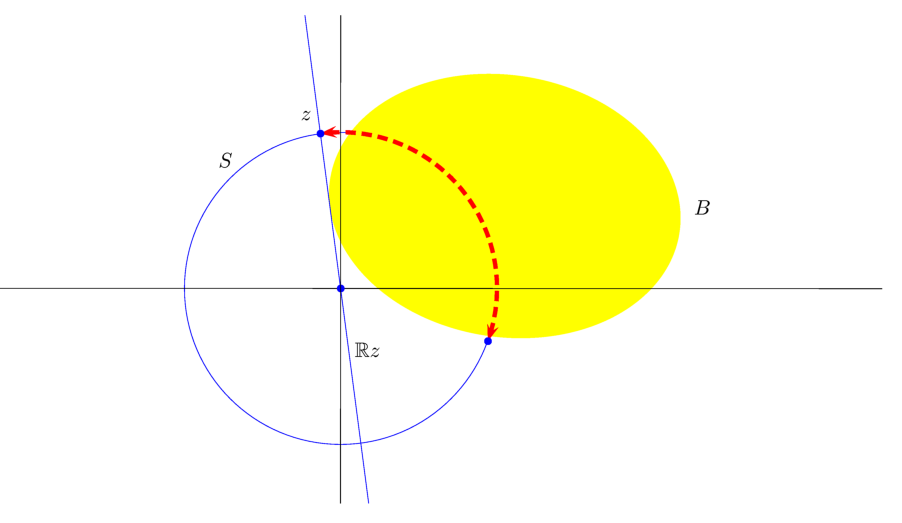
\includegraphics[scale=.7]{rys1}
  \caption{Przykład do uwagi \ref{uw1_r}}
  \scriptsize{ $p(B)$ jest reprezentowane przez czerwoną przerywaną linię.}
\end{figure}
\end{proof}
\begin{uwaga}
  Hiperpłaszczyzna $\left(\textrm{\textit{ang.} hyper\Plane}\right)$ $H$ w~przestrzeni unormowanej $(X,\|\cdot\|)$ jest zbiorem $H= x+Y$, gdzie $Y$ jest podprzestrzenią liniową $X$ kowymiaru 1.
	Jeśli $Y$ jest linowe, to $\overline{Y}$ też. Skoro $\overline{H}=x+\overline{Y}$ i kowymiar $Y=1$, to $\overline{Y} = Y$ albo $\overline{Y} = X$. Z tego wynika, że hiperpłaszczyzna musi być domknięta lub gęsta w $X$.
\end{uwaga}
\begin{twr}[S.~Mazur]
  \index{Twierdzenie!Mazura}
  \label{maz}
	Niech $(X,\|\cdot\|)$ będzie przestrzenią unormowaną. Ponadto niech $L\subset X$ będzie podprzestrzenią liniową oraz $C\subset X$ otwartym zbiorem wypukłym w~$X$ rozłącznym z~$L$. Wtedy istnieje domknięta hiperpłaszczyzna $H$ zawierająca $L$ oraz rozłączna z~$C$.
\end{twr}
%	\emph{W~$(\mathcal{L},\subseteq)$  jest  porządek częściowy, więc działa lemat Kuratowskiego--Zorna}
\begin{proof}
	Niech $\mathcal{L}$ będzie rodziną wszystkich podprzestrzeni liniowych $X$ zawierających $L$ i~rozłącznych z~$C$.
	Wtedy $L \in \mathcal{L}$. Jeśli $\varphi \subset \mathcal{L}$ jest łańcuchem w~$(\mathcal{L},\subseteq)$, wtedy $\bigcup \varphi\in \mathcal{L}$.
	Z Lematu Kuratowskiego--Zorna istnieje element maksymalny $M$ w~$(\mathcal{L}, \subseteq)$.
	\begin{enumerate}[(A)]
		\item $(X,\|\cdot\|)$ jest przestrzenią liniową nad \R.
		
$M\in \mathcal{L}$ więc $\overline{M} \in \mathcal{L}$ więc z maksymalności $M=\overline{M}$, czyli $M$ jest domknięta.
			Pokażemy ponadto, że kowymiar $M=1$. Przypuśćmy przeciwnie -- wówczas istnieje przestrzeń liniowa $E\subset X$ taka, że $\dim E =2$ i~$E\cap M=\{0\}$.
			Wtedy $B=(C+M)\cap E$ nie zawiera 0.
			$B$ jest zbiorem wypukłym i~otwartym w~$E$ (z~konstrukcji $B$ w~powyższym wierszu).
			Więc istnieje $F\subset E$ -- jednowymiarowa podprzestrzeń taka, że $B\cap F = \emptyset$.
			Wtedy $(M+F)\cap C= \emptyset $ ($m+f=c$, $c-m=f$, $c-m \in M+C$ nie możliwe).
			Zatem $M+F \in \mathcal{L}$ i~$M+F$ jest ściśle większe od $M$ w~sensie inkluzji, co daje sprzeczność.
		\item $(X,\norm)$ jest nad \C.~Rozważmy $X_\R$ opisaną w~(A), wtedy $M$ jest hiperpłaszczyzną w~$X_{\R}$.
			Zatem $H=M\cap iM$ jest hiperpłaszczyzną w~$X$, rozdzielną z~$C$. $L\subset H$ ponieważ $iL=L$.
	\end{enumerate}
\end{proof}
% SEBLIS - koniec korekty
\begin{twr}[Hahn--Banach]
  	\index{Twierdzenie!Hahna--Banacha}
	$(X,\norm)$ -- przestrzeń unormowana nad \K.~Niech $Y\subset X$ będzie podprzestrzenią liniową i 
	$f:Y\to \K$ będzie funkcjonałem liniowym takim, że $|f(y)| \le \|y\|$ dla $y\in Y$.
	Wtedy istnieje funkcjonał liniowy $\tilde{f} :X \to \K$ taki, że $\tilde{f}|_Y = f$ i~$|\tilde{f}(x)|\le \|x\|$
\end{twr}
\begin{proof}
  Jeśli $f=0$ to $\tilde{f} = 0$. Jeśli $f\not =0$ to weźmy $u \in Y$  takie, że $f(u)=1$.\par
	Niech $C =\{ x \in X: \|x - u\|<1\}$. Pokażemy, że $C\cap \ker f = \emptyset$.\par
	Weźmy $y\in Y$.
	$|f(y)-f(u)|=|f(y-u)|\le \|y - u\|$. Jeśli $y\in C$ to  $f(y) \not =0$.
	Z~{twierdzenia Mazura(\ref{maz})} istnieje w~$X$ hiperpłaszczyzna $H$ taka, że $\ker f\subset H$ i $H\cap C = \emptyset$.
	Kontynuując dowód, ponieważ $u\in C$ to $u \not \in H$ więc $X=H\oplus \K u$.
	Niech $\tilde{f}(x+\lambda u) = \lambda$ dla $x\in H$ i~$\lambda \in \K$. Wtedy $\tilde{f}$ jest  przedłużeniem $f$.\\
	Ponadto, wiemy, że $\|x +\lambda u\|\ge |\lambda| = |\tilde{f} (x+\lambda u)|$ Co znaczy, że $\|x\| \ge |f(x)|$ dla $x\in X$
\end{proof}
\begin{uwaga}
	Niech $(X,\norm)$ -- unormowana przestrzeń rzeczywista. Niech $Y\subset X$ będzie podprzestrzenią liniową.
	$C\subset X$ -- otwarty wypukły podzbiór $X$ taki że $C \cap Y \not = \emptyset $ Niech $f:Y\to \R$ funkcjonał liniowy taki, ze  
	$f$ jest dodatni na $C\cap Y$. Wtedy istnieje $\tilde{f} : X \to \R$ który jest przedłużeniem $f$ i~$\tilde{f}$ jest ściśle dodatni na $C$.
\end{uwaga}
\begin{proof}
	Będziemy używać twierdzenia Mazura: Niech $L= Y \cap \ker f$ wtedy $L\cap C = \emptyset$. 
	Istnieje hiperpłaszczyzna $H$ w~$X$ taka, że $L\subset H$ i~$H\cap C = \emptyset$.
	Weźmy $u \in C \cap Y$. Wtedy $Y = \ker f \oplus \R u$ i~$X = H\oplus \R u$.
	Zdefiniujmy $\tilde{f} = (h+\lambda u) = \lambda f(u)$. I~jest dobrze. 
\end{proof}
% Ja nie wiem jakie tu powinien być dokładnie tytuł.
\section{Twierdzenie o~reprezentacji  Riesza dla nieujemnych funkcjonałów liniowych na C[a,b]}
$C[a,b]$ -- przestrzeń funkcji ciągłych na $[a,b]$ w~$\R$.\par
Liniowy funkcjonał $\varphi:C[a,b]\to \R$ jest nieujemny jeśli $\varphi(f)\ge 0$ dla $f \ge 0)$
\begin{twr}[F.~Riesz]
  \index{Twierdzenie!Riesza}
Niech $\varphi:C[a,b]\to \R$ liniowy, nieujemny  funkcjonał.
Istnieje wtedy miara Borelowska $\mu$ na $[a,b]$ taka, że $\varphi(f) = \int_{[a,b]} f \dd \mu$ dla $f\in C[a,b]$.
\end{twr}
Dla ułatwienia skupimy się teraz na $[a,b]=[0,1]$.
\begin{lem} \label{lem:Riesz1}
  Niech $F\colon[0,1]\to [0,+\infty)$ będzie funkcją niemalejącą. Niech $F_l(t) = \lim\limits_{s\to t^-} F(s)$ dla $t\in[0,1]$. 
  Istnieje wtedy miara Borelowska $\mu$ na $[0,1]$
  taka, że $\mu\left( [0,t) \right) = F_{l}(t)$ i $\mu\left( [0,1) \right) = F(1)$.
\end{lem}
\begin{proof}
	%	\texttt{rysunek} \\ tu miał być rysunek  f jako funkcji schodkowej.
			Niech $G\colon[0,F(1)] \to [0,1]$ będzie funkcją zdefiniowaną wzorem: $G(y) = \inf\{x: F(x) \ge y\}$.
			Jak łatwo zauważyć funkcja $G$ jest niemalejąca oraz  $[0,F_l(t)) \subset G^{-1}[0,t)\subset [0,F_l(t)]$.
			Zdefiniujmy $\mu$ na $[0,1]$ przez $\mu(A) = \lambda(G^{-1}(A))$ gdzie $\lambda$ jest miarą Lebesgue'a.
\end{proof}
\begin{uwaga}
	Niech $I=[0,1]$, $\psi: l_\infty (I,\R)\to \R$ liniowy, nieujemny  funkcjonał. 
	Istnieje wtedy  przeliczalny zbiór $J\subset I$ i~miara Borelowska $\mu$ na $I$ taka, że $\psi\left(\chi_{[0,t)} \right) = \mu[0,t)$ 
		$\psi \left( \chi_{[s,t)}  \right)  = \mu[s,t)$ i~$\psi(\chi_{[0,1]}) = \psi(1) = \mu[0,1]$.
\end{uwaga}
\begin{proof}
	Niech $F(t) = \psi\left( \chi_{[0,t)} \right)$ dla $t<1$ i~$F(1) = \psi(1)$.
	Jeśli $s<t$ to $\chi_{[0,s)} \le \chi_{[0,t)}$ więc $\psi\left( \chi_{0,s)} \right) \le \psi \left( \chi_{[0,t)} \right)$
		bo $\psi (\chi_{[0,t)} ) - \psi (\chi_{[0,s)}) = \psi(\chi_{[s,t)}) >0$.
	%  Ponieważ $\psi$ jest nieujemne to 
	Czyli $F$ jest niemalejące i~mamy $\mu$ jak w~poprzednim lemacie (\ref{lem:Riesz1}).\\
	Niech $J= \{t: F_l (t) < F(t)\}$ -- zbiór punktów skoku jest przeliczalny. 
	Wtedy $\mu$ i $J$ mają takie własności jakie chcieliśmy. 
\end{proof}
\begin{uwaga}
	Niech $\varphi:C[0,1] \to \R$ jest liniowym, nieujemnym funkcjonałem i~$\varphi \not = 0$ wtedy  $\varphi(f) >0 $ dla każdego $f>0$ 
\end{uwaga}
\begin{proof}
	Każdą funkcję $u \in C[0,1]$ można przedstawić jako różnicę $u=u^+-u^-$ nieujemnych funkcji ciągłych $u^+ = \max(u,0)$ i~$u^- = \max(-u,0)$.
	Dlatego, jeśli $\varphi\not = 0$ to istnieje $v\ge 0$ dla którego $\varphi(v)>0$.
	Weźmy $f>0$ gdzie $\inf f = \delta >0$. Mamy $\frac{\delta}{\|v\|}v\le f$. Z~liniowości $\varphi$ mamy $\varphi(f)\ge \frac{\delta}{\|v\|}\varphi(v)>0$
\end{proof}
\begin{proof}[Dowód twierdzenia Riesza]
	Niech $\varphi: C[0,1] \to \R$ będzie  nieujemnym funkcjonałem linowym.
	Rozważmy $\left( C[0,1],\norm_\infty \right)$ jako liniową podprzestrzeń $\left( l_\infty (I,\R),\norm_\infty \right)$
	Niech $C=\{ u\in l_\infty (I,\R): \inf_{t \in I} u(t) >0\}$. Wtedy $C$ jest otwartym wypukłym zbiorem w~$l_\infty(I,\R)$. \par
%	$C\cap C[0,1] = \{ f \in C[0,1]: f>0\}$.\par
	Z~Uwagi 1.4.4 funkcjonał $\varphi$ jest dodatni na $C \cap C[0,1]$.\par
	Z~Uwagi 1.3.6.	istnieje ciągły liniowy funkcjonał $\psi:\l_\infty(I,\R) \to R$ taki, że $\psi$ jest dodatni na $C$ i~jest przedłużeniem $\varphi$\par
	Jeśli $v\ge 0$ dla $v \in l_\infty (I,\R)$ to $u\in \overline{C}$ więc $\psi(v)\ge0$.\par
	Niech $\mu$ będzie miarą jak w~Uwadze 1.4.3.
	Musimy sprawdzić dla $f\in C[0,1]$, ze $\varphi(f) = \int_{[0,1]}f \dd \mu$.
	Ustalmy $\varepsilon>0$. Dopóki $f$ jest jednostajnie ciągła możemy zastąpić $[0,1]$ przez punkty $0<t_1<\ldots<t_n<1$
	takie, że oscylacja $f$ na przedziałach $[0,t_1),\ldots [t_{n-1},t_{n}), [t_n 1]$ jest mniejsza niż $\varepsilon$\par
	Niech $g$  będzie funkcją schodkową zdefiniowaną: 
	$$g= f(0)\cdot \chi_{[0,t_1)} + \sum_{i=1}^{n-1}f(t_i) \chi_{[t_i,t_{i+1}} + f(t_n) \chi_{[t_n,1]}$$
	Wtedy $|f-g| \le \|f-g\|_\infty<\varepsilon$ więc $-\mathbf{1} \varepsilon < f-g < \mathbf{1} \varepsilon$, 
	czyli $\psi(f-g) <\varepsilon \psi(\mathbf{1})$
 	\begin{multline}
	\left|\varphi(f) - \int_{[0,1]} f \dd \mu\right| = \left| \psi(f) - \psi(g) +\psi(g) - \int_{[0,1]} f \dd \mu \right|
	\le \left| \psi(f-g)\right| + \int_{[0,1]} \left| g - f \right| \dd\mu
	\nonumber
  \end{multline}
  Ale oba elementy z~prawej można oszacować przez $\varepsilon\varphi(\mathbf{1})$ więc $\left|\varphi(f) - \int_{[0,1]} f \dd \mu\right|<2\varepsilon\varphi(\mathbf{1})$.
  Co z~dowolności wyboru $\varepsilon$ kończy dowód.
\end{proof}

\section{Ograniczone operatory liniowe}
\begin{de}
Niech $(X,\norm)$ i~$(Y,\norm)$ będą unormowanymi przestrzeniami liniowymi nad tym samym ciałem \K.
Odwzorowanie liniowe (operator liniowy) $T\colon X \to Y$ jest ograniczone jeśli:
$$\| T\| = \sup \{\|T(x)\|\colon x \in B_x\} < \infty$$

Oznaczmy przez $B(X,Y)$ przestrzeń liniowa wszystkich ograniczonych operatorów z~$X$ do $Y$.

$(B(X,Y) \norm)$ -- przestrzeń unormowana \\
$(B(X,\K), \norm)$ przestrzeń dualna do $(X,\norm)$ oznaczana przez $(X^*,\norm)$
\end{de}
\begin{uwaga}
	\begin{enumerate}[(A)]
		\item Niech $T\in B(X,Y)$ wtedy $\forall x\in X: \|T(x)\| \le \|T\| \cdot \|x\|$. 
			Norma operatora to najmniejsze takie $M$, że $\|T(x)\| \le M \cdot \|x\|$ dla każdego $x\in X$.
		\item Odwzorowanie liniowe $T\colon X \to Y$ jest ciągłe wtedy i~tylko wtedy gdy jest ograniczone.\\
			$\Rightarrow$ $\|Tx-Ty\| = \|T(x-y)\| \le \|T\| \cdot \|x - y\|$ wiec $T$ jest jednostajnie ciągła.\\
			$\Leftarrow$ Jeśli $T$ jest ciągła w~punkcie 0. Weźmy $\varepsilon=1$ wtedy istnieje $\delta>0$ taka, że $\|x\|\le \delta$.
			wtedy $\|Tx\|\le 1$.
			Dla $x\not =  0$ $\left\|T\left( \delta \frac{x}{\|x\|} \right)\right\|\le 1$, czyli $\|T(x)\|\le \frac{1}{\delta}\|x\|$.

	\end{enumerate}
\end{uwaga}
\begin{ex}	
%	\begin{enumerate}[(A)]
%		\item $(C_0)^* = l_1$
%		\item $(l_1)^* = l_\infty$
%\end{enumerate}
	\textup{(A)} $(c_0)^* = l_1$ i~\textup{(B)}$(l_1)^* = l_\infty$
\end{ex}
\begin{proof}[Dowód (A)]
  Chcemy zdefiniować liniową izometrię $S\colon (c_o)^* \overset{\textrm{na}}{\longrightarrow} l_1$.
	Oznaczmy przez $e_n = (0,0,\ldots,0,1,0,\ldots)$ gdzie jedynka jest na $n$-tym miejscu.\par

	Niech $S(\varphi) = \left( \varphi(e_1), \varphi(e_2),\ldots \right)$ dla $\varphi\in (c_0)^*$. 
	Chcemy pokazać, że $S(\varphi)\in l_1$ oraz, że $S$ jest izometrią. \par
	Zaczniemy od pokazania pierwszego warunku.
	Niech $\varphi\in (c_0)^*, \varphi(e_i) = c_i$ i~ $v_n = \frac{\overline{c_1}}{|c_1|}e_1 + \ldots+ \frac{\overline{c_n}}{|c_n|}e_n \in c_0$ wtedy $\|v_n\|_\infty=1$. Więc:
	$$|\varphi(v_n)| = \left| \frac{\overline{c_1} c_1}{|c_1|}+\ldots+\frac{\overline{c_n} c_n}{|c_n|} \right|= |c_1| +\ldots + |c_n| \le \|\varphi\|\cdot \|v_n\|_\infty = \|\varphi\|$$
	Ponieważ $\|\varphi\|$ jest skończone to stąd dostajemy, że $S(\varphi) \in l_1$.\\
	
	Od razu dostaliśmy, że $\|S(\varphi)\|_1 \le \|\varphi\|$, więc wystarczy pokazać  nierówność w~drugą stronę, aby wykazać, że $S$ jest izometrią.
	Weźmy dowolny ciąg $x=(x_1,x_2,\ldots)\in c_0$ taki, że $\|x\|_\infty$. Wtedy $x_1e_1+\ldots+ x_n e_n  \to x$ w~$c_0$, więc $\lim\limits_n( x_1\varphi(e_1)+ \ldots +x_n\varphi(e_n)) = \varphi(x)$
	Dlatego:
	$$|\varphi(x)|\le \sum_{n=1}^\infty |\varphi(e_n)| =\|S(\varphi)\|_1$$
	A~ponieważ zachodzi to dla dowolnego $\|x\|_\infty \le 1$ to dostajemy nierówność $\|\varphi\| \le \|S(\varphi)\|_1$.
	
	Tak więc wiemy, że $S$ jest liniową izometrią. Trzeba jeszcze wykazać, ze jest surjekcją. Ale każdy ciąg $y= (c_1,c_2,\ldots)\in l_1$ definiuje funkcjonał liniowy $\varphi$ wzorem
	$\varphi(x) = \sum c_i x_i$. 

%	$\varphi(x) = \sum_i x_i c_i$  gdzie $x=(x_1, x_2, \ldots)$ to $S(\varphi) = (c_1,c_2,\ldots)$.\par
%	Niech $\varphi \in (c_0)^*$ i~$\varphi(e_i) = c_i$. 
%	Niech $v_n = \frac{\overline{c_1}}{|c_1|}e_1 + \ldots+ \frac{\overline{c_n}}{|c_n|}e_n \in c_0$ wtedy $\|v_n\|_\infty =1$.	Więc: 
%	$$|\varphi(v_n)| = \left| \frac{\overline{c_1} c_1}{|c_1|}+\ldots+\frac{\overline{c_n} c_n}{|c_n|} \right|= |c_1| +\ldots + |c_n| \le \|\varphi\|\cdot \|v_n\|_\infty = \|\varphi\|$$
%	Stąd dostajemy, że $S(\varphi) \in l_1$ i~$\|S(\varphi)\|_1 \le \|\varphi\|$.

%		\item Pokażemy, że sstnieje liniowa izometia $S\colon(C_0)^* \to l_1$. Taka, że dla $\varphi \in (c_0)^*$ zachodzi $\|S(x)\| = \|x\|$.
%			Dla każdego $x= (x_1,x_2,\ldots) \in c_0$ $\varphi(x) = \sum_i x_i c_i$
%			Wtedy $S(\varphi) = (c_1,c_2,\ldots) \in l_1$.\\
%			Niech $e_n =(0,0,\ldots,0, \underset{n}{1},0 \ldots) \in c_0$ wtedy $x_1 e_1 + \ldots+ x_n e_n = (x_1,\ldots,x_n,0, \ldots)$.
%			Niech $s(\varphi) = (\varphi(e_1), \varphi(e_2), \ldots)$.
%			Pozostaje pokazać, ze (1) $S(\varphi) \in l_1$ i~(2) $\|\varphi\| = \|S(\varphi)\|_1$\\
%			Aby sprawdzić pierwszy warunek: Niech $S(\varphi) = (c_1, c_1, \ldots)$ gdzie $c_i = \varphi(e_i)$.
%			Niech $v_n = \frac{\overline{c_1}}{|c_1|}e_1 + \ldots+ \frac{\overline{c_n}}{|c_n|}e_n \in c_0.$ wtedy $\|v_n\|_\infty =1$.
%			Więc $|\varphi(v_n)| \le \|\varphi\|\cdot \|v_n\|_\infty = \|\varphi\|$ 
%			gdzie $\varphi(v_n) = \frac{\overline{c_1} c_1}{|c_1|}+\ldots+\frac{\overline{c_n} c_n}{|c_n|}= |c_1| +\ldots+|c_n|$.\par
%			Przy okazji udowodniliśmy nierówność $\le$ dla drugiego warunku \par
%			Dla nierówności $\|\varphi\| \le \|S(\varphi\|_1$. 
%			Niech $x= (x_1,x_2, \ldots) \in c_0$. Ciąg $x_1e_1 + \ldots + x_n e_n \longrightarrow x$ w~$c_0$. 
%			Wiec $\varphi(x_1e_1 + \ldots + x_n e_n) \to x$ bo $\sum x_n c_n = \varphi(x)$ \\
%			Jeśli $\|x\|_\infty \le 1$ wtedy $\|S(\varphi)\|_1 = \sum |c_n| \ge |\varphi(x)|$ 
%			Finalnie $S$ jest na. 
%
%			\texttt{Do przeczytania i~korekty}
\end{proof}
Dowodu (B) nie było na wykładzie.
\begin{uwaga}
	Dla każdego $\varphi\in (C[a,b])^*$ istnieją skończone miary Borelowskie $\mu, \nu$ takie, że 
	$\varphi(f) = \int_{[a,b]} f \dd\mu - \int_{[a,b]} f \dd \nu$ i~$\|\varphi\| = \mu[a,b]+ \nu[a,b]$
\end{uwaga}
\begin{uwaga}[konsekwencje twierdzenia Hahna\dywiz Banacha]
	Niech $Y$ będzie liniową podprzestrzenią przestrzeni unormowanej $(X,\norm)$.
	Niech $\varphi\in Y^*$ wtedy istnieje $\psi \in X^*$ takie, że $\psi|_Y = \varphi$ i $\|\psi\| = \|\varphi\|$.
	
\end{uwaga}
\begin{proof}
Weźmy $f= \frac{1}{\|\varphi\|} \varphi$ wtedy 
$|f(x)| = \frac{1}{\|\varphi\|}|\varphi(x)| \le \frac{1}{\|\varphi\|}\|\varphi\|\cdot \|x\| = \|x\|$.
Wtedy istnieje $\tilde{f} \colon X \to K$ taki, że $\tilde{f}|_Y = f$ i~$ |\tilde{f}(x) | \le \|x\| $
\end{proof}
\section{Przestrzenie Banacha}
\begin{de}
	Przestrzeń unormowana $(X\norm )$ która jest zupełna w~metryce $d(x,y) = \|x- y\|$ jest przestrzenią Banacha.
\end{de}
\begin{ex}
	\begin{enumerate}[(A)]
		\item Dla dowolnego zbioru $S$ $\left( l_\infty(S,\K),\norm_\infty \right)$ jest przestrzenią Banacha. 
		\item Dla przestrzeni unormowanej  $(X,\norm)$ i~przestrzeni Banacha $(Y,\norm)$ przestrzeń $\left( B(X,Y), \norm \right)$ 
			jest przestrzenią Banacha.
		\item Przestrzeń $(c_0, \norm_\infty)$ jest przestrzenią Banacha. Więc $(l_1,\norm_1)= (c_0)^*$ jest Banacha  z~(B).
	\end{enumerate}
\end{ex}
\begin{uwaga}
	Jeśli $(X,\norm)$ jest przestrzenią Banacha i~dla wektorów $x_n \in X$ zachodzi $\sum_n \|x_n\| < +\infty$ wtedy 
	$\sum_n x_n$ jest zbieżny i~do tego dla każdej permutacji $\sigma\colon \N\to\N$ zachodzi $\sum_n x_{\sigma(n)} = \sum_n x_n$
\end{uwaga}
\subsection{Przestrzenie $(B(X),\norm)$ ograniczonych endomorfizmów przestrzeni Banacha}
Niech $S,T \in B(X)$ wtedy $\|S\circ T\| \le \|S\| \cdot \|T\|$ bo 
$\|S\circ T (X) \|= \| S(T(x))\| \le \|S\|\cdot \|T(x)\| \le \|S\| \cdot \|T\| \cdot \|x\|$.

\begin{twr}
	Niech $(X,\norm)$ będzie przestrzenią Banacha i~niech $T\in B(X)$ taki, że $\|T\| <1$. Wtedy $I_X - T$ jest odwracalny i~
	$\left( I_X - T  \right)^{-1} = \sum_{n=1}^\infty T^n$.
\end{twr}
\begin{proof}
	Wiemy, że $\|T^n\|\le \|T\|^n$, wiec $\sum_{n=0}\|T^n\| \le \sum_{n=0} \|T\|^n = \frac{1}{1-\|T\|}$ czyli
	szereg $\sum_{n=0}^\infty T^n$ jest zbieżny. 
	Chcemy sprawdzić,że $I_X=(I_X -T)  \left( \sum_{n=0}^\infty T^n \right)= \sum_{n=0}^\infty \left( (I_X-T) T^n \right)=
	(I_X-T)+(T-T^2)+\ldots=I_X$
\end{proof}
\begin{wn}
	Niech $(X,\norm)$ będzie przestrzenią Banacha. Niech $GL(X)$ będzie zbiorem wszystkich odwracalnych operatorów w~$B(X)$.
	Wtedy zbiór $GL(X)$ jest otwarty w~$(B(X),\norm)$ 
\end{wn}
\begin{proof}
	Weźmy $T\in GL(X)$ i $r= \frac{1}{\|T^-1\|}$. Niech $S\in B(x)$ takie, że$\|S-T\|<r$.
	Pokażemy, że $S \in GL(X)$. \\
	Mamy $\|T^{-1}(S-T)\| \le \|T^{-1}\|\cdot\|S - T\| <1$ więc $I-T^{-1}(S - T)$ jest odwracalny.
	Ale $S= T(I+T^{-1}(S - T ))\in GL(X)$. 
\end{proof}
\begin{lem}
	Niech $(X,\norm)$ będzie przestrzenią Banacha. Niech $T \in B(X)$.
	Niech $\delta(T) = \inf\{ \|Tx\|: x \in S_x\}$ 
	\begin{enumerate}[(i)]
		\item Jeśli $\delta(T) = 0$ wtedy $T$ jest nieodwracalny.
		\item $\delta(T) >0$ wtedy $\im T =TX$ jest domknięty w~$X$ oraz $T\colon X \to \im X$ jest homeomorfizmem liniowym.
	\end{enumerate}
\end{lem}
\begin{proof}
	\begin{enumerate}[(i)]
		\item Jeśli $ \delta(T) =0$ wtedy istnieje ciąg $x_n \in S_x$ taki, że $T{x_{n}}\to 0$ co jest sprzeczne 
			z~istnieniem ograniczonego $T^{-1}$.  Ponieważ $ T^{-1 }T x_n = x_n \to T^{-1}o = 0$ dla $x_n \in S_X$ 
		\item Jeśli $\delta(T)>0$ to $\ker(T) = \{0\}$ wiec $ T\colon X \to \im T$ ma liniową odwrotność
			$S\colon \im T \to X$ taką, że $T\circ S = I_{\im T}$.
			Pokażemy teraz ograniczoność $S$. W~tym celu weźmy $x\not = 0$ wtedy $\left\|T\left( \frac{x}{\|x\|} \right)\right\|\ge \delta(T)$
			Czyli $\|Tx\| \ge \delta(T) \|x\|$ więc wiemy że istnieje $y\in \im T$ takie, że $x=Sy$ i~mamy 
			$\|y\|\ge \delta(T) \|Sy\|$.
			Dostajemy stąd ograniczenie $\|Sy\| \le \frac{1}{\delta(T)}\|y\|$ dla $y\in \im T$.\\
			Sprawdźmy teraz czy $\overline{\im T} = \im T \in X$.
			Weźmy dowolny ciąg $y_n \in \im T$ taki że $y_n \to x$.  Wtedy $(y_n)_n$ jest ciągiem Cauchego. 
			$\|S{y_n} - S{y_m}\|=\|S(y_n - y_m)\|\le \|S\| \cdot \|y_n -y_m\|$ wiec ciąg $(S y_n)_{n=1}^\infty$ jest ciągiem Cauchego.
			Z~zupełności przestrzeni $X$ wynika, że $S y_n \to z$ więc $T S y_n \to T z$ czyli $y_n \to Tz$ 
	\end{enumerate}
\end{proof}
\begin{de}
	Niech \spac będzie przestrzenią Banacha nad \K.~Niech $T \in B(x)$.
	\begin{enumerate}
		\item Widmem nazwiemy $\sigma(T) = sp(T) = \{ \lambda \in \K : T -\lambda I_X \textrm{ jest nieodwracalny}\}$ 
		\item $\lambda\in K$ jest wartością własną $T$ jeśli istnieje $x\not  =0$ taki, że $Tx = \lambda x$. 
			$X$ jest wektorem  własnym zwiazanym z~$\lambda$
	\end{enumerate}
\end{de}
\begin{uwaga}
	Niech $T\colon \K^n \to \K^n$ wtedy $sp(T) = \{\lambda: \ker(T-\lambda I) \not = 0\} = \{\lambda :\lambda \textrm{ jest wartością własną} \}$
\end{uwaga}
%\begin{uwaga}
	%\texttt{Tu była jakaś notatka}
%\end{uwaga}
\begin{ex}
	Niech $T\colon C[0,1] \to C[0,1]$ taki że $Tf(t) = t\cdot f(t)$ wtedy $sp(T) = [0,1]$ ale $T$ nie ma wartości własnych.
\end{ex}
\begin{proof}
	Ustalmy $\lambda \in [0,1]$ Pokażemy, że $T -\lambda I$ jest nieodwracalne. Wystarczy, że sprawdzimy, że $\delta(T-\lambda I) =0$.
	Dla ustalonego $\lambda$ bierzemy ciąg funkcji $u_n$ taki że (od pewnego, odpowiednio dużego $n$):
	$$u_n(t) = \left\{
		\begin{array}[]{ll}
		 	0 & \textrm{dla } t \in \left[0,\lambda-\frac{1}{n}\right] \cup \left[ \lambda+\frac{1}{n}, 1 \right]\\
			1 + n(x -\lambda) & \textrm{dla } t \in \left[ \lambda-\frac{1}{n},\lambda \right]\\
			1+n(\lambda -x)	& \textrm{dla } t \in \left[ \lambda,\lambda+\frac{1}{n} \right]
		\end{array}\right.
	$$
	\begin{figure}[h]
	  \centering
	  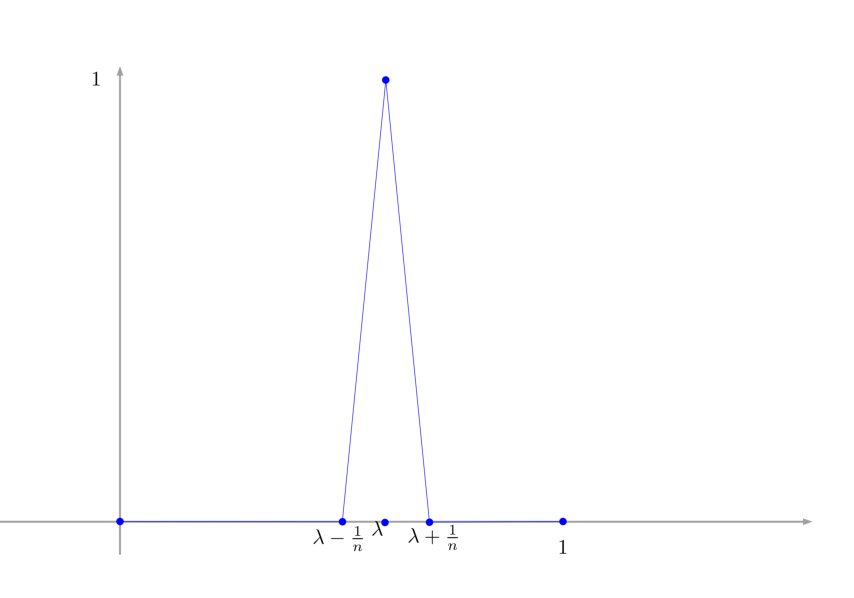
\includegraphics[scale=.7]{rys2}
	  \caption{wykres funkcji $u_n$}
	\end{figure}

	Wtedy $\|u_n\|_\infty=1$. Weźmy $|(T- \lambda I) u_n(t)| = |tu_n(t) - \lambda u_n(t)| = |t-\lambda| |u_n(t)| \le \frac{1}{n}$.
	Więc $\delta(T-\lambda I)  = \inf \{ \|T-\lambda I )u \|_\infty : \|u\|_\infty =1\} = 0$ 
	%\texttt{tu czegoś brakuje,ale zostało szybko starte :(}
	Na mocy lematu 1.6.7 (i) $\lambda \in sp(T)$ czyli udowodniliśmy, że $sp(T) = [0,1]$. \par
	Załóżmy, że $Tu = \lambda u$ dla pewnego $\lambda \in [0,1]$ i~$u \in C[0,1]$.
	Wtedy $tu(t) = \lambda u(t) $ dla $t\in[0,1]$ więc $u(t) = 0$ dla $t\not = \lambda$. Z~ciągłości $u$ wynik że $u=0$.
\end{proof}
\begin{uwaga}
	Niech \spac będzie przestrzenią Banacha, niech $t\in B(x)$ wtedy $sp (T)$ jest domkniętym zbiorem 
	$\{\lambda : |\lambda| \le \|T\|\}$ więc $sp(T)$ jest zbiorem zwartym.
\end{uwaga}
\begin{proof}
	Obierzmy $|\lambda| >\|T\|$. Wówczas mamy $\left\| \frac{1}{\lambda} T\right\|<1$, więc operator  $I- \frac{1}{\lambda}T$ jest odwracalny, czyli
	także $T - \lambda I = \lambda\left( I -\frac{1}{\lambda}T \right)$ jest odwracalny, wiec $\lambda\not \in sp(T)$. \\
	Skoro $GL(X)$ jest otwarty, a odwzorowanie $\lambda \mapsto T - \lambda I$ jest ciągłe, to $sp(T)$, jako 	przeciw obraz domkniętego zbioru $B(X) \setminus GL(X)$, 
	jest domknięty.
\end{proof}
\section{Zwarte operatory liniowe}
\begin{de}
	Operator $T\colon X\to X$, gdzie \spac jest przestrzenią Banacha, jest zwarty jeśli $\overline{T(B_X)}$ jest zbiorem zwartym. Wówczas w szczególności jest on ograniczony: $T\in B(X)$.
\end{de}
\begin{twr}[F.~Riesz, J.~Schauder]
	Niech $T\colon X \to X$ będzie operatorem zwartym na nieskończenie wymiarowej przestrzeni Banacha \spac. Wtedy:
	\begin{enumerate}
		\item $0\in sp(T)$
		\item Każdy niezerowy element $sp(T)$ jest wartością własną $T$ 
	\item dla każdego $\varepsilon>0$ istnieje  skończenie wiele $\lambda \in sp(T)$ takich wiele $|\lambda|\ge\varepsilon$ 
	\end{enumerate}
\end{twr}
\begin{lem}
	\label{lem:173}
	Niech $T\in B(X)$ będzie zwartym izomorfizmem. Wtedy operator $T-I_X$ jest odwracalny wtedy i~tylko wtedy gdy $\ker (T-I_X) =\{0\}$ 
\end{lem}
\begin{proof}
	$\Rightarrow$ oczywiste (odwracalny operator ma zerowe jądro).\par
	Niech $\ker(T-I_X) = \{0\}$. Chcemy $\delta(T-I_X) = \inf \{ \|(T-I_X) x\|: x\in S_X\} >0$\par
	\underline{Jeśli nie} to istnieją $x_n \in S_X$ taki, że $(T-I_X)x_n \to 0$.
	Ze zwartości $T$Istnieje podciąg  $n_1<n_2<\ldots$ taki, że $T{x_{n_i}} \to x$ czyli ponieważ $T x_{n_1} - x_{n_i} \to 0$
	więc $x_{n_i} \to x$ i~$T x_{n_i} \to Tx$ zatem $x=Tx$ i~$(T-I_X)x=0$, a~ponieważ $\|x\| =1$ to $x\not = 0$ i~$x \in \ker(T -I_X)$
	Czyli sprzeczność\par
	Zatem $T-I_X\colon X \to \im(T - I)$ jest liniowym homeomorfizmem i~$\overline{ \im(T - I)} =  \im(T - I)$.
	Pokażemy, ze $ \im(T - I) = X$\par
	Niech $x_0 = X$ i~$X_{i+1}=(T-I_X)X_i$ wtedy istnieje $i$ takie, że $X_i = X_{i+1}$.\par
	\underline{Jeśli nie} to z~lematu Riesza wybierzemy $x_i \in X_i\cap S_X$ taki, że $\dist(x_i, X_{i+1}) > \frac{1}{2}$ 
	Pokażemy, że jeśli $i<j$ to $\|Tx_i - Tx_j\|\ge \frac{1}{2}$.
	Rzeczywiście : $\|Tx_i - Tx_j\| = \|Tx_i -x_i +x_i -x_j +x_j - T x_j\|=\| x_i -( -\underset{\in X_{i+1}}{(T-I_X)x_i}+ 
	\underset{\in X_{j+1}}{(T-I_X)x_j}+x_j )\|
	\ge \frac{1}{2}$
	Ale $TS_x$ jest zwarte, a~nie ma podciągu zbieżnego.\par
	Niech $i$ - minimalny indeks taki, że $X_i = X_{i+1}$. Jeśli $i>0$ to wybierzmy $x \in X_{i-1}\setminus X_i$.
	Wtedy $(T-I_X) x \in X_i = X_{i+1}$. Wiec dla pewnego $y \in X_i$ mamy $ (T-I_x)x = (T-I_X)y$ stąd $x-y \in \ker(T-I_X)$ i~$x-y \not =0$
\end{proof}
\begin{proof}[Dowód tw. F.~Riesz, J.~Schauder]
	\begin{enumerate}[(i)]
			\item $T(B_X)$ jest zwarty więc brzegowy w~$X$ (Kula nie jest zwarta w~przestrzeni nieskończenie wymiarowej)
				$T(X) = T\left( \bigcap_n nB_X \right) = \bigcap_n n T(B_x) \not=X$ (na mocy twierdzenia Baire'a) czyli $T$ nie jest odwracalny.
			\item Niech $\lambda \in spT$ czyli $T-\lambda I$ jest nieodwracalny. 
				Ale $T-\lambda I = \lambda\left(\frac{1}{\lambda}T - I\right)$.
				Z~lematu \ref{lem:173} $\left( \frac{1}{\lambda}T - I \right)$ ma niezerowe jądro,
				więc jądro $\lambda\left( \frac{1}{\lambda}T - I \right)$ również jest niezerowe, czyli $\lambda$ jest wartością własną.
			\item Załóżmy, że nie. Niech $\lambda_1, \lambda_2,\ldots$ niezerowe wartości własne takie, że $|\lambda_i|>\varepsilon$.
				Niech $y_i \in S_X$ takie, że $Ty_i = \lambda_i y_i$. Wtedy $y_1, y_2,\ldots$ są liniowo niezależne.
				Niech $Y_i = \lin \{y_1,\ldots,y_i\}$.
				Z~lematu Riesza istnieją $x_i \in Y_{i+1} \setminus Y_{i}$, $x_i \in S_X$ i~$\dist(x_i, Y_i) \ge \frac{1}{2}$.
				Pokażemy, że jeśli $i>j$ to $\|T x_i - Tx_j\|\ge \frac{\varepsilon}{2}$.
				Wiemy że $x_i = y+ a y_{i+1}$ dla $y\in Y_i$ wtedy 
				$$Tx_i = Ty + a \lambda_{i+1} y_{i+1} =
				\lambda_{i+1}\left( \frac{1}{\lambda_{i+1}}Ty +a y_{i+1} \right) = 
				\lambda_{i+1}\left( \frac{1}{\lambda_{i+1}}Ty +x_i -y) \right)$$
				$$\|Tx_i - Tx_j\| = |\lambda_{i+1}|\left\| \texttt{\ldots} \right\| \ge \frac{\varepsilon}{2}$$
		\end{enumerate}
\end{proof}
\begin{uwaga}
	Niech $T\in B(X)$ będzie zwarty i~\spac będzie przestrzenią Banacha to dla $\lambda \in sp(T) \setminus \{0\}$ 
	$\ker (T - \lambda I)$ jest skończenie wymiarowe. (ze zwartości obrazu kuli)
\end{uwaga}
\chapter{Przestrzenie Hilberta}
Przestrzenią Hilberta nazwiemy przestrzeń liniową $X$ nad $\C$ wyposażoną w iloczyn skalarny 
$\langle \cdot,\cdot \rangle \colon X \times X \to \C$,
taki że przestrzeń $X$ jest zupełna w~metryce wyznaczonej przez normę, wyznaczoną przez iloczyn skalarny.
\section{Iloczyn skalarny}
\begin{de}
	Iloczynem skalarnym (lub wewnętrznym)  na zespolonej przestrzeni liniowej jest funkcją $\langle \cdot, \cdot \rangle \colon X\times X \to\C$
	taka, że:
	\begin{enumerate}[(1)]
		\item dla każdego $y\in X$ funkcja $x \to \langle x,y \rangle$ jest liniowa
		\item $\langle x,y \rangle = \overline{\langle y,x \rangle}$
		\item $\langle x,x \rangle\ge 0$ i~$\langle x,x \rangle=0$ wtedy i~tylko wtedy gdy $x=0$ 
	\end{enumerate}
	Zauważmy, że z~(1) i~(2) wynika, że $\langle x,\lambda y \rangle = \overline{\lambda}\langle x,y \rangle$
\end{de}
\begin{ex}
	\texttt{Tu w~skrypcie są przykłady}
\end{ex}

%\par\texittt{tu powinno być przypomnienie iloczynu skalarnego nad $\C$}
\begin{twr}[Nierówność Cauchego\dywiz Schwarza] Dla każdego iloczynu skalarnego na przestrzeni zespolonej:
	$|\langle x,y \rangle| \le \sqrt{\langle x, x \rangle} \sqrt{\langle y, y \rangle}$
\end{twr}
\begin{proof}
%	\texttt{Tak jakoś zamuliłem, może dopiszę}
	Dla $y=0$ sytuacja jest oczywista. Weźmy więc $y\neq 0$ i~niech $\lambda = -\frac{\langle x,y \rangle}{\langle y,y \rangle}$.
	Wtedy $0\le\langle x+\lambda y,x+\lambda y \rangle = \langle x,x \rangle + |\lambda|^2 \langle y,y \rangle + \lambda\langle y,x \rangle + \overline{\lambda}
	\langle x,y \rangle = \langle x,x \rangle - \frac{|\langle x,y \rangle|^2}{\langle y,y \rangle}$
	Co już daje nam nierówność.
\end{proof}
\begin{uwaga}
	Dla dowolnego iloczynu skalarnego nad liniową przestrzenią  zespoloną $X$ zachodzi:
	\begin{enumerate}[(A)]
		\item ``Prawo równoległoboku'' $\|x\|^2+\|y\|^2 = \frac{1}{2}\left( \|x+y\|^2 + \|x-y\|^2 \right)$ 
		\item $\langle x,y \rangle = \frac{1}{4}\left( \|x+y\|^2 - \|x -  y\|^2  + i \|x+iy\|^2 - i\|x-iy\|^2\right)$
			Zatem $(X,\langle \cdot,\cdot \rangle_X)$, $(Y,\langle \cdot,\cdot \rangle_Y)$. Niech  $T\colon X\to Y$ będzie przekształceniem liniowym. 
			$T$ zachowuje produkty skalarne wtedy i~tylko wtedy, gdy $T$ zachowuje normę, wiec $\langle Tx,Ty \rangle_Y = \langle x,y \rangle_X$.
	\end{enumerate}
\end{uwaga}
\begin{ex}
	Niech $L_2(\mu) = L_2 (\Omega,\mathcal{B},\mu)$. Niech $\mathcal{B}$ będzie $\sigma$ ciało podzbiorów $\Omega$. $\mu$ jest dana miarą.
	Niech $f\colon \Omega \to \C$. Definiujemy klasę abstrakcji $[f] = \{ g: \Omega \to \C : ??, \mu\{x; f(x) \not = g(x) \} =0\}$.
	Wtedy $[f]+[g] = [f+g]$ i~$\lambda[f] = [\lambda f]$.\par
	Niech $L_2 (\Omega,\mathcal{B} ,\mu) = \{[f]: f\textrm{ jest całkowalna z kwadratem}\}$.
	Wtedy $\langle [f],[g] \rangle = \int_\Omega = f \overline{g} \dd \mu$ i~$\|[f]\|_2 = \left( \int_\Omega |f|^2 \dd\mu \right)^{\frac{1}{2}}$\par
	Potrzebujemy sprawdzić, że przestrzeń $(L_2 (\mu) ,\norm_2)$ jest zupełna.
	\begin{enumerate}[(A)]
		\item Niech $0\le g_1 \le g_2 \le \ldots$, $g_i\colon \Omega \to [0,+\infty)$ mierzalne oraz $\int_\Omega g_i^2 \dd\mu \le M$ 
			Wtedy dla $t\in \Omega$ $g_i(t) < \infty$ prawie wszędzie i~dla $g = \lim_i g_i $ 
			(określone prawie wszędzie) i~$\int_\Omega g^2 \dd \mu \le M$. 
			Używając Twierdzenia Lebesgua o~zbieżności zmajoryzowanej $g_i^2 \to h$ i~$\int_\Omega h \dd \mu \le M$ więc weźmy $g=\sqrt{h}$.
		\item Niech $([f_n])_{n=1}^\infty$ będzie ciągiem Cauchego w~$L_2(\mu)$ 
			Istnieją 
			$$\begin{array}{lll}
				n_1 & \|f_{n_1} - f_i \|_2 < 1 & \textrm{dla } i\ge n_1\\
				n_2>n_1 & \|f_{n_2} - f_i  \|_2 < \frac{1}{2} & \textrm{dla } i \ge n_2\\
				n_{k+1} > n_k & \|f_{n_{k+1}} - f_i \|_2 < \frac{1}{2^k}& \textrm{dla } i\ge n_{k+1}
			\end{array}$$
			Niech $g_k = |f_{n_1}| + |f_{n_2} - f_{n_1}| + \ldots+ |f_{n_{k+1}} - f_{n_k}|$.
			Wtedy $0\le g_1 \le g_2\le\ldots$.
			Zauważmy, że $\|g_k\|_2 \le \|f_{n_1}\|_2 + \|f_{n_2} - f_{n_1}\|_2+\ldots+\|f_{n_{k+1} - f_{n_k}}\|_2 \le \|f_{n_1}\|_2+2$.\par
			Z~podpunktu $(A)$: $g_k \nearrow g$ (prawie wszędzie) i~$g$ jest całkowalna z~kwadratem prawie wszędzie. 
			Ciąg $f_{n_{k+1}}$ jest zbieżny (punktowo), a~więc $f_{n_k} \to f$ prawie wszędzie  jeśli $|f_{n_k}|^2 \to |f|^2$ prawie wszędzie.
			(ciąg $[f_n])_n$ jest Cauchego i~$\|f_n\|_2$ są wspólnie ograniczone)
			Ponieważ, $\int_\Omega |f|^2 \dd \mu \le \infty$ to $[f]\in \L_2(\mu)$ \par
			Sprawdzimy, że w~$L_2(\mu)$ $[f_{n_k}]\to[f]$.
			Scałkujmy $\sqrt{\int_\Omega |f_{n_k} - f|^2 \dd \mu} = \|f_{n_k}-f\|_2 \le \|f_{n_k}\|_2 + \|f\|_2\le M$
			i~jeśli $|f_{n_k}|^2  \to 0$ prawie wszędzie to $\|f_{n_k}-f\|_2 \to 0$. \par
			Jeśli $([f_n])_n$ jest ciągiem Cauchego to $[f_n] \to [f]$ w~$L_2(\mu)$
	\end{enumerate}

\end{ex}
\begin{de}
	Niech $(H,\langle \cdot,\cdot \rangle)$ będzie przestrzenią Hilberta jeśli $\langle \cdot,\cdot \rangle$ jest takim iloczynem skalarnym na $H$, że dla 
	$\|x\| = \sqrt{\langle x,x \rangle}$, $(H,\norm)$ jest przestrzenią Banacha. 
\end{de}
Czyli $(L_2(\mu),\|\cdot\|_2)$ jest przestrzenią Hilberta.
\begin{ex}
	Weźmy $(l_2,\norm_2)$ (ciągi sumowalne z~kwadratem). Zdefiniujmy iloczyn skalarny $\langle x,y \rangle = \sum_{i}^{}x_i \overline{y_i}$.
	Wtedy $\|x\| = \sqrt{\langle x,x \rangle} = \left( \sum_{i}^{}|x_i|^2 \right)^\frac{1}{2}$
\end{ex}
\begin{twr}
	Niech $(H,\scal)$ będzie przestrzenią Hilberta. Niech $C\subset H$ będzie domkniętym, wypukłym zbiorem.
	Wtedy, dla każdego $x\in H$ istnieje unikalny wektor $P_C(x) \in C$ taki, że $\|x-P_C(x) \| = \dist(x,C)$
\end{twr}
\begin{proof}
	Ustalmy $x$. Dla dowolnych $u,v$ z~reguły równoległoboku: 
	$$\|x - u\|^2 + \|x - v\|^2 = \frac{1}{2}\left( \|2x - (u+v)\|^2 + \|u-v\|^2 \right)$$.
	Weźmy $u_n\in C$ takie, że $\|x-u_n\| \to \dist(x,C)$.
	Musimy sprawdzić, że $(u_n)_{n=1}^\infty$ jest ciągiem Cauchego.
	$$\|x-u_n\|^2 + \|x-u_m\|^2 = \frac{1}{2}\left( \|2x -(u_n+u_m)\|^2 + \|u_n - u_m\|^2 \right)$$
	$$\frac{1}{2} \underset{\ge 0}{\|u_n-u_m\|^2} = \underset{\to \dist(x,C)}{\|x-u_n\|^2} + \underset{\to \dist(x,C)}{\|x-u_m\|^2} - 
	2 \left( \underset{\to \dist(x,C)}{\left\|x-\frac{(u_n-u_m)}{2}\right\|^2} \right) \longrightarrow 0$$
	Wiec $(u_n)_n$ jest ciągiem Cauchego i~ze zupełności $u_n \to u$, $\overline{C} = C$ i~$u\in C$ 
	i~$\|x -u\|= \dist(x,C)$. Wynika z~tego ,że $u$ jest jedynym taki wektorem. Ustalmy $u = P_C(x)$.
\end{proof}
\chapter{Zadania od Toruńczyka i~inne dodatki}
Być może coś się tu pojawi. Zapraszam chętnych. 
%\chapter{Piosenka}
%Dlaczego? Bo tak:\par\nopagebreak
\newpage
\section*{Przestrzenie Liniowe}
\textit{Autor: YanPL} Na melodie \textit{Hiszpańskich Dziewczyn}  \par\nopagebreak
%\small
{\begin{tabular}{ll}
{Żegnajcie nam dziś, przestrzenie} liniowe,	  &  e C H7 \\ 
Żegnajcie nam dziś, macierze ich baz				  &  e G D \\ 
Ku całkom Riemanna już ruszać nam pora				  &  C D e \\ 
Lecz do tych przestrzeni wrócimy nie raz			  &  C H7 e \vspace{0.8eM}\\ 

		{I smak waszych baz przestrzenie} liniowe		  &  e G D \\ 
		W noc ciemną i złą nam będzie się śnił		  &  e G D \\ 
		Leniwie popłyną granice punktowe			  &  C D e \\ 
		Wspomnienie ciał waszych przysporzy nam sił	  &  C H7e \vspace{0.8eM}\\ 

Niedługo ujrzymy szeregi funkcyjne \\ 
ekstremów lokalnych w przedziale (a b) \\ 
Dowody twierdzenia w notatkach z wykładów \\ 
lecz znów na kolokwium nam wyjdzie to źle \vspace{0.8eM}\\ 

Niedługo poprawek wyniki rozkwitną \\ 
i każdy się dowie czy w końcu to zdał \\ 
Bo na analizie niepewny jest człowiek \\ 
Co pływa myślami wśród rzutów i ciał \vspace{0.8eM}\\ 

Zabłysną nam bielą porządki liniowe \\ 
I wykład upłynie wśród legend i bajd \\ 
moc klasy abstrakcji relacji zerowej \\ 
Po zbiorach niepustych zrobimy znów rajd \vspace{0.8eM}\\ 

Niedługo zbiór liczb naturalnych zabłyśnie \\ 
Ciągami co nigdy nie zbiegną do zer \\ 
I moc continuum nad nami zawiśnie \\ 
Bijekcją nas rzuci rekinom na żer \vspace{0.8eM}\\ 

Zawiniem do portu przy sekcji studenckiej \\ 
Lecz tam jak w tawernie gdy skończy się rum \\ 
Najchętniej by mocno Ci dali po gębie \\ 
Uciekaj więc prędko nim zmiażdży Cię tłum \vspace{0.8eM}\\ 

Więc gdy się zaciągniesz na studia na MIMie \\ 
By płynąć ku wiedzy przez huk morskich fal \\ 
Wśród przeszkód i przygód Ci życie upłynie \\ 
A lekiem na szkorbut okaże się GAL \\ 
\end{tabular}}
\printindex
\end{document}
